% ============================================================================
% moved_from_paper2.tex
%
% Holding file. Material lifted out of paper2/main.tex during the 2026-09-07
% merge of Paper 2 into paper/main.tex (Paper A), per paper/RESTRUCTURE_PLAN.md
% ("What moves to Paper B").  Nothing here is \input by any paper yet; drop the
% pieces into paper3/main.tex when that document is written.
%
% Labels have been given a "p2" prefix so they cannot clash with Paper A's.
% Figure paths are relative to paper3/ and assume ../results/... as before.
%
% Source of record for the original text: paper2/main.tex (unmodified,
% archival), sections listed against each block below.
% ============================================================================


% ----------------------------------------------------------------------------
% 1. Cross-generation Qwen3 -> Qwen3.5 comparison
%    Source: paper2/main.tex, subsection "Cross-Generation Comparison"
%    (\label{sec:crossgen}, lines 518-555 of the archival file), complete with
%    its figure include and caption.
%    Paper B rationale: Paper B covers generations 3.6/3.8 and prompts across
%    generations; this matched-pair Qwen3 -> Qwen3.5 comparison is the first
%    rung of that ladder, and it needs the properly seeded Qwen3 replication
%    that Paper B will run.
% ----------------------------------------------------------------------------

\subsection{Cross-Generation Comparison}
\label{p2:sec:crossgen}

Figure~\ref{p2:fig:crossgen} compares Qwen3 and Qwen3.5 at matched
parameter counts using Q4\_K\_M quantization.

\begin{figure}[t]
\centering
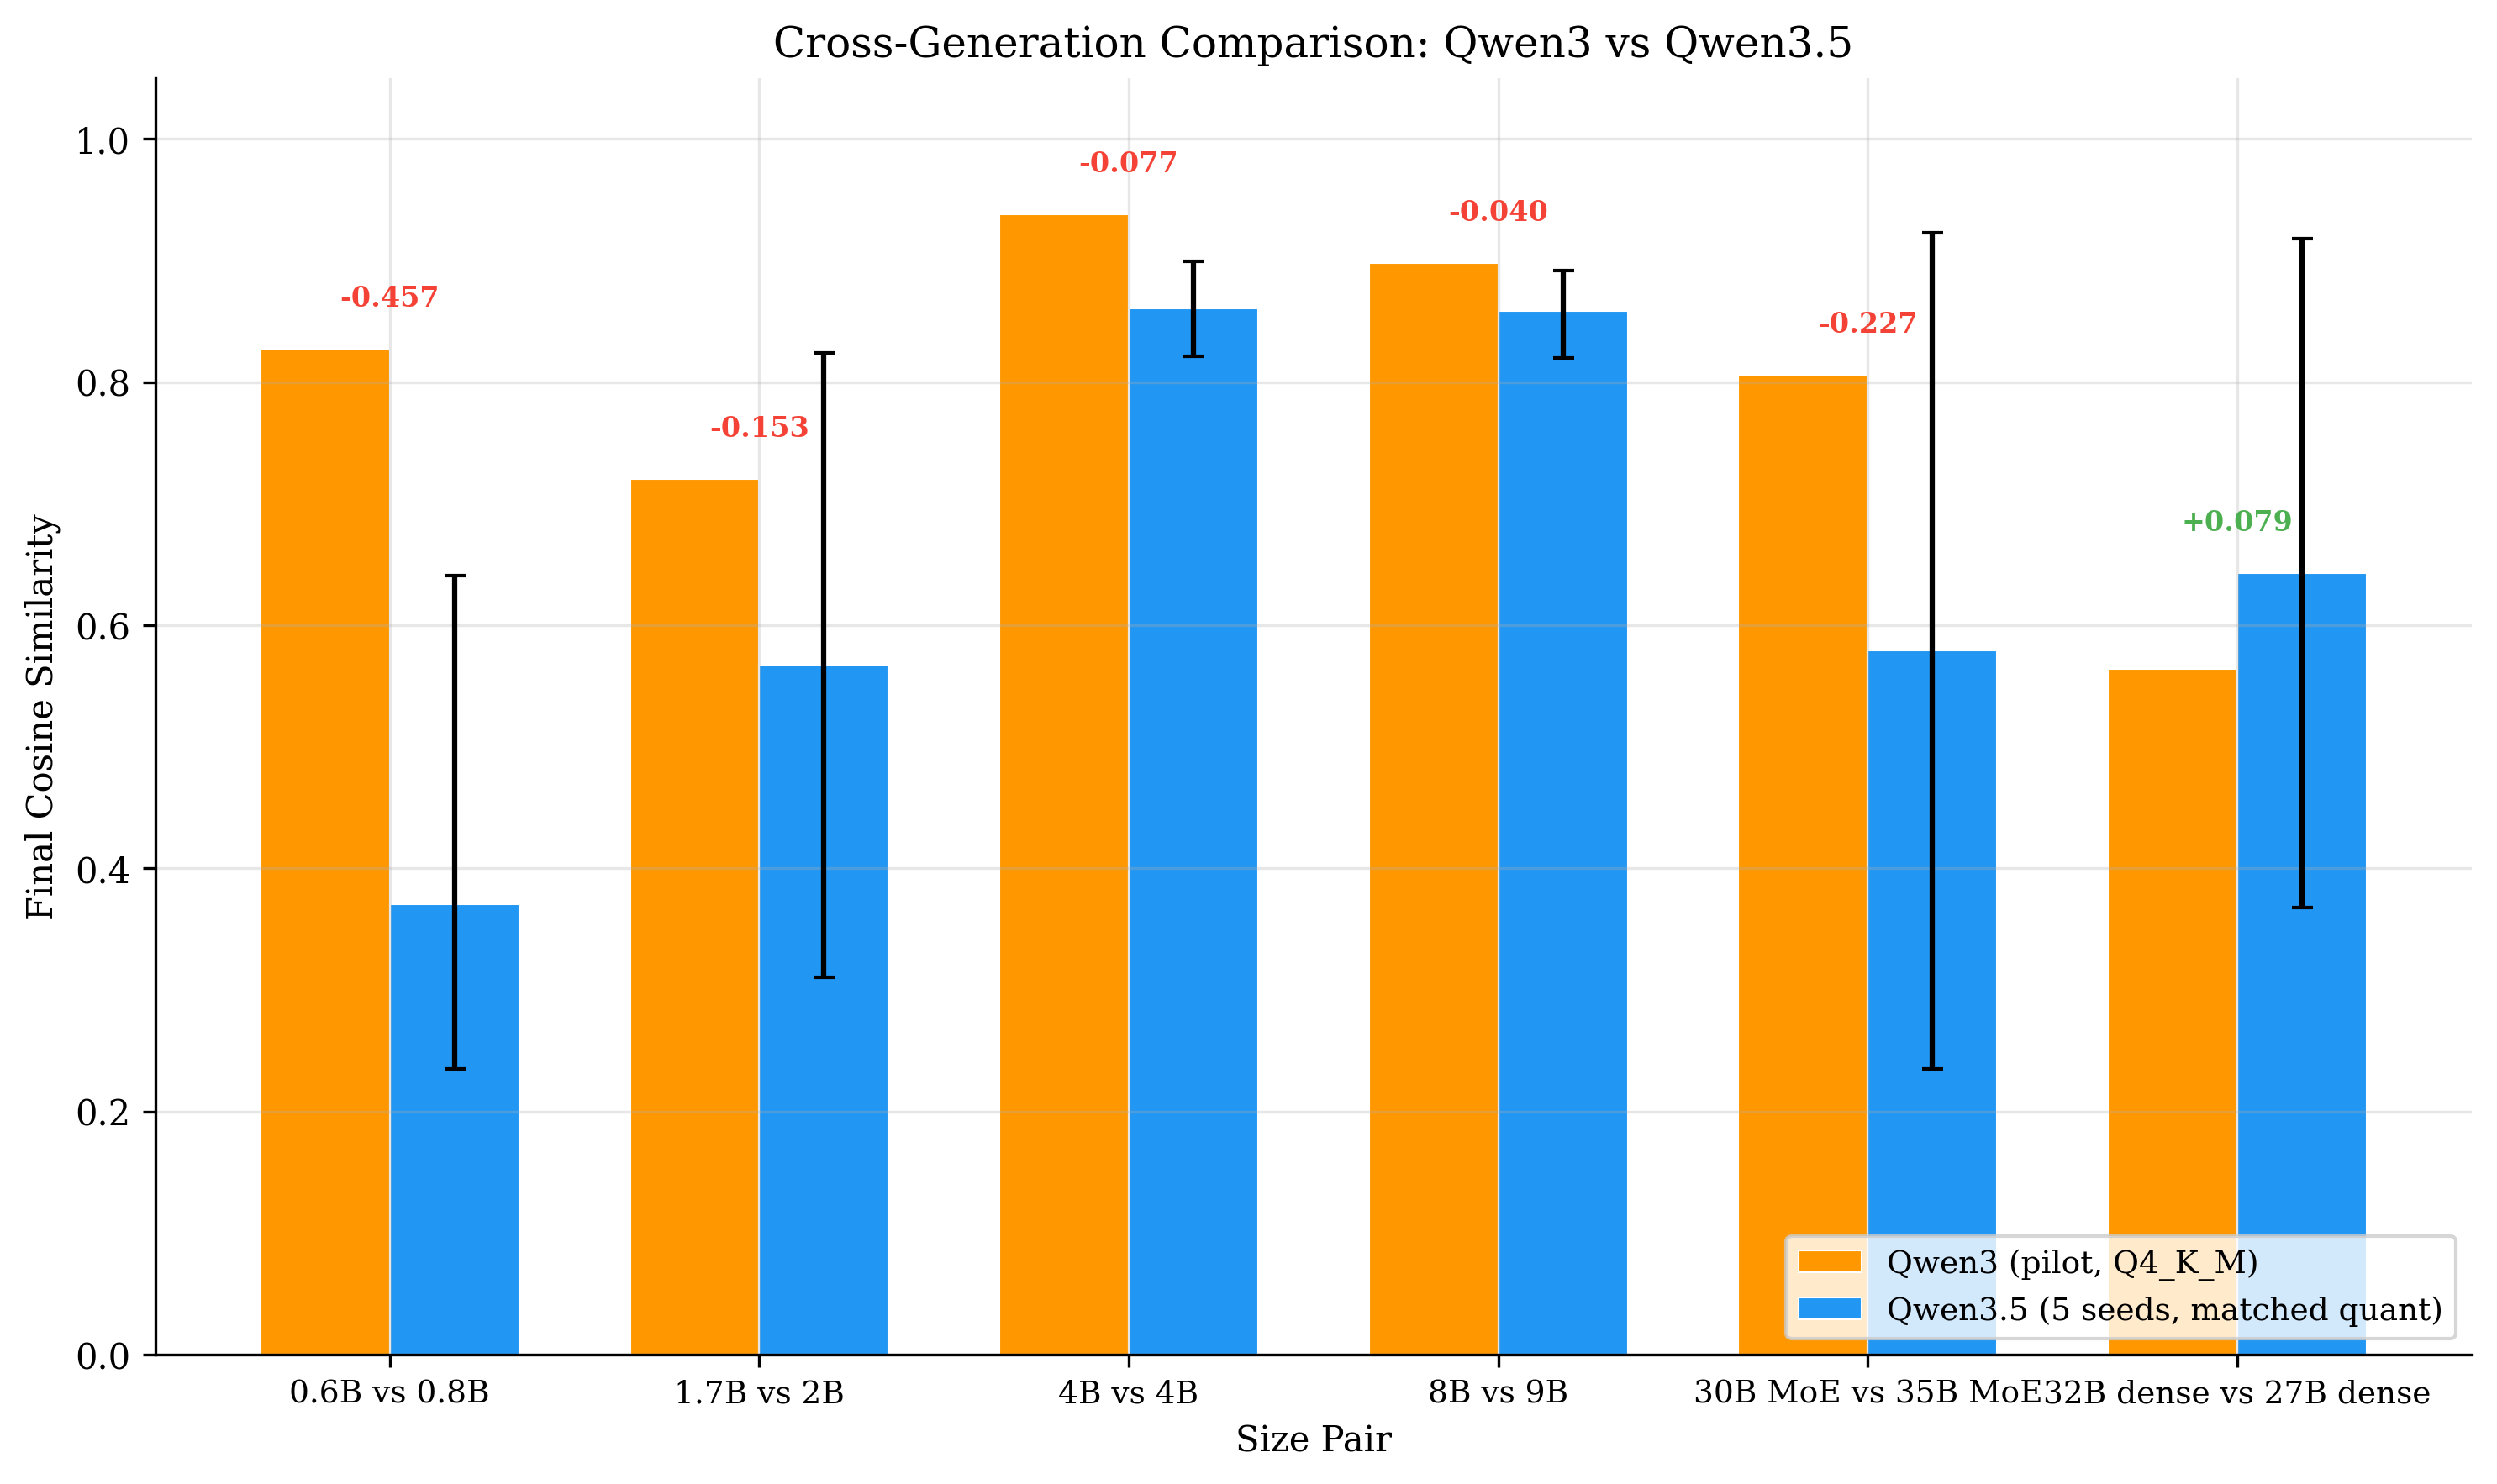
\includegraphics[width=0.85\textwidth]{../results/qwen35_paper_figures/fig10_cross_generation.png}
\caption{Cross-generation comparison: Qwen3 (pilot, single run) vs.\
  Qwen3.5 (up to 5 completed chains, matched quantization). The Qwen3
  bars carry \emph{no} error bars because each is a single unreplicated
  run from the cross-family pilot; only the Qwen3.5 bars have bootstrap CIs.}
\label{p2:fig:crossgen}
\end{figure}

\paragraph{Dense model improvement at 27B.}
The 27B dense Qwen3.5 model is the only matched pair in which Qwen3.5
leads: 0.643 vs.\ Qwen3's 32B dense at 0.564 ($+$0.079). Its bootstrap
interval, [0.368, 0.918], comfortably contains the Qwen3 value, so this
is a directional observation rather than a demonstrated improvement.

\paragraph{MoE models regress.}
The 35B MoE (Qwen3.5, 0.579) trails the 30B MoE (Qwen3, 0.806) by
$-$0.227. Because the Qwen3.5 value is depressed by two chains that
collapse to the empty-output floor, this gap reflects a difference in
failure \emph{rate} rather than in gradual fidelity loss.

\paragraph{Small model regression.}
Below 4B parameters, Qwen3.5 regresses compared to Qwen3: the 0.8B model
(0.370) trails Qwen3's 0.6B (0.827) by $-$0.457, and the 2B (0.567)
trails Qwen3's 1.7B (0.720) by $-$0.153. The 4B and 9B pairs are close
to parity ($-$0.077 and $-$0.040). Taken together, five of six matched
pairs favour Qwen3. We caution strongly that the Qwen3 arm comes from a
single unreplicated pilot run with no confidence interval at all, while
the Qwen3.5 means are averaged over up to five chains; the comparison
should be read as motivating a properly seeded replication, not as
evidence of a generational regression.

% Accompanying limitation, source: paper2/main.tex Limitations item 4.
% \item \textbf{Qwen3 comparison is unbalanced.} The Qwen3 data come from
%       single pilot runs, while Qwen3.5 data have 5 seeds. The
%       cross-generation comparison should be interpreted cautiously.

% Accompanying contribution/conclusion items dropped from Paper A:
%   contribution 5: "A cross-generation comparison between Qwen3 and Qwen3.5
%     at matched parameter counts (Section~\ref{sec:crossgen})."
%   conclusion item 5: "A cross-generation comparison in which five of six
%     matched pairs favour Qwen3 over Qwen3.5, which we report as a call for a
%     properly seeded replication given that the Qwen3 arm is a single pilot
%     run."


% ----------------------------------------------------------------------------
% 2. Empty-output / thinking-overhead hypothesis
%    Sources: paper2/main.tex "Stability threshold at 4B" paragraph (the
%    mechanistic sentences only) and Limitations item 8 ("Empty outputs and
%    thinking overhead").
%    Paper B rationale: this is the hypothesis Paper B tests directly, by
%    re-running with thinking disabled and by instrumenting the reasoning-token
%    budget. Paper A now reports the failure mode descriptively only, in its
%    "Runaway thinking as a failure mode" subsection, without asserting the
%    mechanism.
% ----------------------------------------------------------------------------

% (a) Mechanistic sentences removed from the 4B-threshold paragraph:

Many of these low-similarity scores result from the model returning
\emph{empty} output strings---the API returns a successful response with no
content. The most likely explanation is that the model's internal thinking
process (Qwen3.5 models use a think-before-responding architecture) consumes
the entire generation budget on reasoning tokens, leaving nothing for the
final answer. This failure mode is consistent across seeds and becomes more
frequent as chain inputs degrade through drift.

% (b) Limitations item, verbatim (as a list item):

\begin{itemize}[leftmargin=*]
  \item \textbf{Empty outputs and thinking overhead.} Several models
        (particularly 0.8B and 27B Q4\_K\_M) produce empty output strings
        in a substantial fraction of iterations. We attribute this to
        Qwen3.5's think-before-responding architecture consuming the
        generation budget on internal reasoning tokens, but we cannot
        fully rule out serving-layer issues (e.g., Ollama silently
        truncating). The empty outputs are recorded as data and chains
        continue with the previous non-empty message, but this recovery
        mechanism may mask the true depth of drift.
\end{itemize}

% Suggested citations when this material is written up in Paper B:
%   yang2025qwen3       -- the hybrid thinking / non-thinking mode itself
%   he2025nondeterminism, zhang2025deterministic, zhao2026corun -- batch
%                          invariance and the seeds-are-samples caveat
%   leviathan2023speculative, chen2023speculative, gloeckle2024multitoken,
%   deepseek2024v3      -- speculative decoding and MTP
% All of these are already present in paper/references.bib.
